\chapter{Einleitung und Motivation}
\label{chapter1}

\section{Einleitung}
\label{chapter1-Einleitung}


\section{Motivation}
\label{chapter1-Motivation}
Von September 2021 bis August 2024 forschen die Hochschule für angewandte Wissenschaften in Hamburg
und die Universität der Bundeswehr München im Rahmen des \emph{HoPE-Projekts} zusammen an Effekten
rund um die Steigerung der Aufmerksamkeit bei der Nutzung von großen, interaktiven Wandbildschirmen,
sogenannten \emph{Ambient Displays}.
Dieser Bereich weist noch einen grundsätzlichen Forschungsbedarf auf.
Im Projekt wird unter anderem der \emph{Honeypot-Effekt} erforscht \citep{unibw_honeypot-effekt_2021}.
Dieser beschreibt in der \ac{HCI} wie Menschen die mit einem System interagieren
weitere Passanten anregen die Interaktion zu beobachten oder sogar an ihr teilzuhaben \citep{wouters_uncovering_2016}.
Der \emph{Honeypot-Effekt} soll bei der Nutzung von \emph{Ambient Displays} im öffentlichen
und halb-öffentlichen Raum in Langzeit-Feldstudien analysiert werden.
Dabei soll auch der Aspekt der Datenerhebung und -analyse weiter ausgebaut werden.
Hierzu muss ein methodisches Rahmenwerk entwickelt werden, welches eine auf Sensordaten-basierende,
automatische und zeitlich uneingeschränkte Evaluation von \emph{Ambient Displays} ermöglicht \citep{unibw_honeypot-effekt_2021}.
Die Sensordaten werden von Body-Tracking-Kameras bereitgestellt.
Konkret wurden im die Wandbildschirme im vorliegenden Datensatz mit Kinect v2 Kameras ausgestattet.
Diese zeichnen die Interaktion von Nutzern mit den Displays auf,
wodurch das Nutzerverhalten zu einem späteren Zeitpunkt ausgewertet werden kann.
Besonders interessant ist, welche Muster sich in den Daten erkennen lassen.
Lässt sich eine Menge von Kategorien identifizieren, die etwas über das Verhalten von Menschen vor Wandbildschirmen aussagt?
Ist die Einteilung in diese Kategorien automatisierbar?
Aufgrund der Größe des vorliegenden Datensatzes ist eine manuelle Durchsicht zur Beantwortung der Fragen nicht möglich.
In dieser Bachelorarbeit wird versucht, dieses Problem mithilfe von deterministischen Algorithmen zu lösen.
Wesentliches Ziel ist die Implementierung eines Systems zur Kategorisierung der vorliegenden Kinect-Bewegungsdaten.
Dieses System wird detailiert beschrieben und anschließend evaluiert.
Dabei soll geklärt werden, welches Verfahren sich am Besten für den genannten Sachverhalt eignet.
Außerdem wird die Frage beantwortet, welches Vorwissen benötigt wird,
um das Verfahren einsetzen zu können (z.B. die Vorgabe von konkreten Templates)
und welche Datenpunkte zur Analyse interessant sind (z.B. Laufpfade oder Engaged-Werte).

\section{Kategorien der Interaktion mit Wandbildschirmen}
\label{chapter1-KategorienInteraktion-Wandbildschirme}
Interaktive digitale Medien sind in der Öffentlichkeit immer präsenter.
Deshalb wird es für Wandbildschirme immer schwieriger die Aufmerksamkeit von vorbeigehenden Menschen zu erregen
und sie zur Interaktion zu animieren.
Diese Herausforderungen können nicht einfach durch verbesserte Hardware oder attraktivere Displays gelöst werden.
Stattdessen muss ein besseres Verständnis zwischen Menschen und deren Nutzung von Technologie geschaffen werden \citep{wouters_uncovering_2016}.
\emph{Ambient Displays} sind große, interaktive Bildschirme im (halb-) öffentlichen Raum, mit denen Nutzer interagieren können.
Es handelt sich meist um ästhetisch ansprechende Displays die Personen mit Informationen versorgen \citep{mankoff_heuristic_2003}.
Für ein verbessertes Verständnis der Interaktion von Personen mit solchen Wandbildschirmen kann eine Kategorisierung erfolgen.
Dazu existieren verschiedenste \emph{Audience Behaviour-Interaktionsmodelle}, wovon im Folgenden zwei näher beschrieben werden.

Das \emph{Audience Funnel Modell} beschreibt, wie Menschen sich um ein großes öffentliches Display versammeln
und von Beobachtern zu Interagierenden mit dem System, und anschließend wieder zu Beobachtern werden.
Menschen neigen dazu verschiedene Phasen der Interaktivität zu durchlaufen,
bevor sie direkt mit dem System interagieren \citep{wouters_uncovering_2016, mai_audience_2018}.
Die einzelnen Phasen des \emph{Audience Funnel} werden in \autoref{fig:AudienceFunnelModel} gezeigt.
Eine der Aufgaben eines Wandbildschirms ist also Aufmerksamkeit auf sich zu ziehen
und den Nutzer zu motivieren mit dem System zu interagieren \citep{mai_audience_2018}.
\citet{mai_audience_2018} verweisen darauf, dass \emph{Ambient Displays} in der Öffentlichkeit
nicht undbedingt der zentrale Punkt der Aufmerksamkeit sind, da sie eigene intrinsische Ziele verfolgen.
Die Herausforderung für Entwickler ist es die Systeme so zu gestalten,
dass sie Aufmerksamkeit erregen, sich aber gleichzeitig nicht gezwungen in den Mittelpunkt stellen.

\begin{figure}[ht]
    \begin{center}
    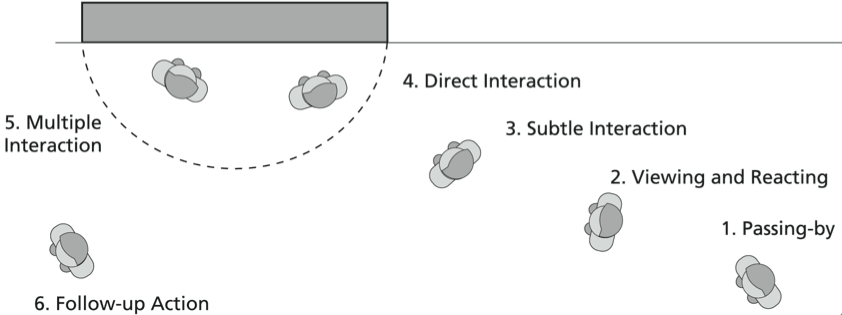
\includegraphics[width=0.9\textwidth]{audience-funnel-model.png}
    \end{center}
    \caption{Audience Funnel Framework. Abbildung aus \citet{mai_audience_2018}.}
    \label{fig:AudienceFunnelModel}
  \end{figure}

Ein zweites Modell wird durch den bereits erwähnten \emph{Honeypot-Effekt} beschrieben.
Dieser Effekt ist ein Einfluss des sozialen Lernens.
Er zeigt, dass Individuen undabhängig von Belohnungen, Bestrafungen oder sozialem Wettbewerb
von der reinen Präsenz oder den Aktivitäten anderer beeinflusst werden.
In der \ac{HCI} wird dies meist erkennbar, indem Passanten sich einem System nähern
und überlegen, ob sie mit ihm interagieren sollen,
nachdem sie anderen Menschen dabei zugesehen haben \citep{wouters_uncovering_2016}.

Eine Einordnung der Bewegungsdaten in solche Kategorien
und eine weiterführende Analyse der Bewegungen kann Aufschluss über das Verhalten von Menschen
vor interaktiven Bildschirmen geben.
Wie bereits erwähnt ist eine Kategorisierung bei einer großen Datenmenge nicht manuell realisierbar.
Im Folgenden werden die Grundlagen der verwendeten Sensorik
und die Struktur des Datensatzes beschrieben.
Aufbauend darauf werden Überlegungen angestellt,
wie eine Implementierung zur Automatisierung der Kategorisierung aussehen kann.


\section{Spezifikation der Kinect}
\label{chapter1-SpezifikationKinect}
Der Xbox 360 Kinect Sensor war eine Revolution im Bereich der erschwinglichen 3D-Erkennungssensorik.
Ursprünglich war er für die Videospiel-Industrie gedacht.
Er wurde aber schon bald von Wissenschaftlern verwendet.
Später folgten weitere Iterationen der Kinect \citep{tolgyessy_evaluation_2021}.
Im vorliegenden Datensatz des \emph{HoPE-Projekts} kam die Kinect v2 für Xbox One zum Einsatz.
Diese Sensorik stellt Farbbilder einer \ac{RGB} Kamera, Tiefenbilder einer Tiefenkamera
und Audiodateien von verschiedenen Mikrofonen zur Verfügung \citep{windows-developer-center_microsoft_corporation_human_2014}.
Besonders die Tiefenkamera hilft zuverlässige Ergebnisse bei der Erkennung von Menschen vor \emph{Ambient Displays} zu erzielen.
\citet{li_time-flight_2014} fassen es wie folgt zusammen.
Die kompakte Größe, die Benutzungsfreundlichkeit,
die stark vereinfachte Hintergrund-Subtraktion im Vergleich zu anderer Sensorik, sowie die hohe Genauigkeit
und die hohe Bildrate machen Tiefenkameras zu einer attraktiven Lösung für ein breites Spektrum an Anwendungen.
Die Kinect v2 verwendet dabei den Ansatz der kontinuierlichen Wellenintensitätsmodulation,
der häufig bei \ac{ToF}-Tiefenkameras zum Einsatz kommt.
Dabei wird das Licht einer Lichtquelle von Objekten im Sichfeld der Kamera zurückgestreut
und die Phasenverzögerung zwischen dem emittierten und dem reflektierten Licht gemessen.
Diese Phasendifferenz wird für jedes Pixel im Bildfeld in einen Entfernungswert umgerechnet \citep{tolgyessy_evaluation_2021}.
Der Sensor kann Tiefenbilder mit einer Auflösung von 512 x 424 Pixeln
und gewöhnliche Farbbilder mit 1920 x 1080 Pixeln aufnehmen \citep{marin_multi-camera_2019}.
Bei der Kinect v2 können bis zu sechs Personen erfasst werden.
Dabei wird die Lage von 25 Skelettpunkten, sowie verschiedene Gesichtsattribute erfasst \citep{windows-developer-center_microsoft_corporation_human_2014}.
\autoref{fig:KinectBodyJoints} zeigt eine Übersicht dieser Punkte. 

\begin{figure}[ht]
  \begin{center}
  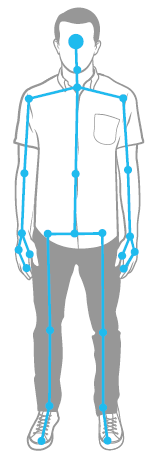
\includegraphics[width=0.1\textwidth]{kinect-body-joints.png}
  \end{center}
  \caption{Skelettpunkte der Kinect v2. Abbildung aus \citet{windows-developer-center_microsoft_corporation_human_2014}.}
  \label{fig:KinectBodyJoints}
\end{figure}


\section{Struktur des vorliegenden Datensatzes}
\label{chapter1-StrukturDatensatz}
Zur Evaluation des implementierten System dient der Kinect-Datensatz des \emph{HoPE-Projekts}.
Hierfür wurden im Jahr 2017 für 18 Wochen zwei Kinect v2 Systeme an einem \emph{Ambient Display} angebracht.
Der Versuchsaufbau kann \autoref{fig:KinectSetup} entnommen werden.
Eine Auswertung des Datensatzes ergab, dass dieser 97.626 Datenpunkte beinhaltet \citep{temiz_konzeption_2022}.
Jeder Datenpunkt enthält mehrere sogenannte Frames.
Dabei handelt es sich um Momentaufnahmen der Kinect-Sensorik.
Zu jedem Datenpunkt liegen verschiedene Dateien vor,
die jeweils den Zeitstempel in Kombination mit einem geeigneten Postfix als Dateinamen tragen:

\begin{itemize}
  \item timestamp.txt
  \item timestamp$\_$bodies.txt
  \item timestamp$\_$summary.txt
  \item timestamp.xef
\end{itemize}

Die Datei \emph{timestamp.txt} enthält folgende Attributwerte:

\begin{enumerate}
  \item Zeitstempel: Zeitpunkt der Aufnahme
  \item KinectId
  \item RecordId: Identifikationsnummer des Records
  \item BodyIndex: Identifikationsnummer der Person
  \item BodyCount: Anzahl der erfassten Personen
  \item Happy: Person ist glücklich
  \item Engaged: Person zeigt Interesse
  \item WearingGlasses: Person trägt eine Brille
  \item LeftEyeClosed: Person hat das linke Auge geschlossen
  \item RightEyeClosed: Person hat das rechte Auge geschlossen
  \item MouthOpen: Person hat den Mund geöffnet
  \item MouthMoved: Person bewegt den Mund
  \item LookingAway: Person schaut nicht zum Kinect-Sensor
  \item Body.HandLeftState: Zustand der linken Hand
  \item Body.HandRightState: Zusand der rechten Hand
  \item X: x-Koordinate des Skelettpunkts SpineShoulder
  \item Y: y-Koordinate des Skelettpunkts SpineShoulder
  \item Z: z-Koordinate des Skelettpunkts SpineShoulder
  \item Distance: Distanz zwischen Kinect-Sensor und Skelettpunkt SpineShoulder
\end{enumerate}

Diese Attribute werden in der Textdatei durch drei Rauten ('\#\#\#') voneinander abgegrenzt.
Die Datei \emph{timestamp$\_$bodies.txt} enthält für jeden Frame die Position aller 25 Skelettpunkte.
\emph{timestamp$\_$summary.txt} zeigt eine kurze Zusammenfassung des Datenpunkts, welche gut von Menschen lesbar ist
und \emph{timestamp.xef} kann genutzt werden, um den Datenpunkt in der Anwendung Kinect Studio zu visualisieren.
Letzlich sind die Einträge sogenannte \emph{Time Series Data}.
Bei diesem Datentyp handelt es sich um geordnete Sequenzen von Datenpunkten,
die über eine gewisse Zeit hinweg aufgenommen werden.
Oft in regelmäßigen Abständen \citep{ali_clustering_2019}.
Jeder Datenpunkt beinhaltet durchschnittlich 355 Frames,
wodurch eine Gesamt-Frameanzahl von 34.687.630 entsteht \citep{temiz_konzeption_2022}.
An der Größe zeigt sich erneut die Notwendigkeit eines Software-Tools zur Auswertung.

\begin{figure}[ht]
  \begin{center}
  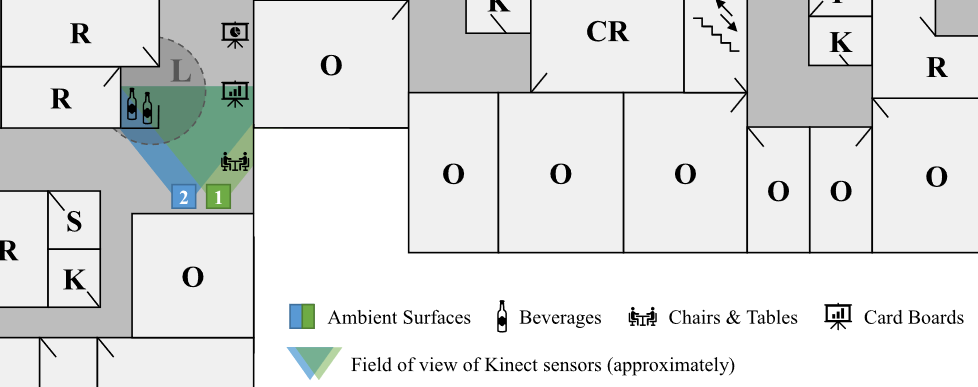
\includegraphics[width=0.8\textwidth]{kinect-setup.png}
  \end{center}
  \caption{Kinect-Setup des Datensatzes. Abbildung von Jan Schwarzer ToDo} %%todo
  \label{fig:KinectSetup}
\end{figure}